\documentclass{article}
\usepackage[paperwidth=360pt,paperheight=190pt,margin=0pt,noheadfoot]{geometry}
\usepackage{tikz}
\usetikzlibrary{calc}

\definecolor{ink}{RGB}{28,41,56}
\definecolor{axis}{RGB}{100,116,139}
\definecolor{grid}{RGB}{203,213,225}
\definecolor{curve}{RGB}{30,64,175}
\definecolor{teal}{RGB}{13,148,136}
\definecolor{tealfill}{RGB}{176,227,219}
% Integral diagrams use cyan for the under-estimate and yellow for the
% over-estimate.  At half opacity their common region is the same green as in
% the signed sin(pi*x)/x diagram, including below the axis.  Orange is only a
% finite correction or an unresolved middle gap.
\definecolor{cyan}{RGB}{7,128,84}
\definecolor{cyanfill}{RGB}{0,160,90}
\definecolor{yellow}{RGB}{170,142,0}
\definecolor{yellowfill}{RGB}{254,243,199}
\definecolor{orange}{RGB}{234,88,12}
\definecolor{orangefill}{RGB}{254,215,170}
\definecolor{purple}{RGB}{126,34,206}
\definecolor{yellowedge}{RGB}{202,138,4}
\definecolor{projection}{RGB}{148,163,184}
\colorlet{under}{cyan}
\colorlet{underfill}{cyanfill}
\colorlet{over}{yellow}
\colorlet{overfill}{yellowfill}
\colorlet{gap}{orange}
\colorlet{gapfill}{orangefill}

\pagestyle{empty}
\setlength\parindent{0pt}
\setlength\topskip{0pt}
\begin{document}
\noindent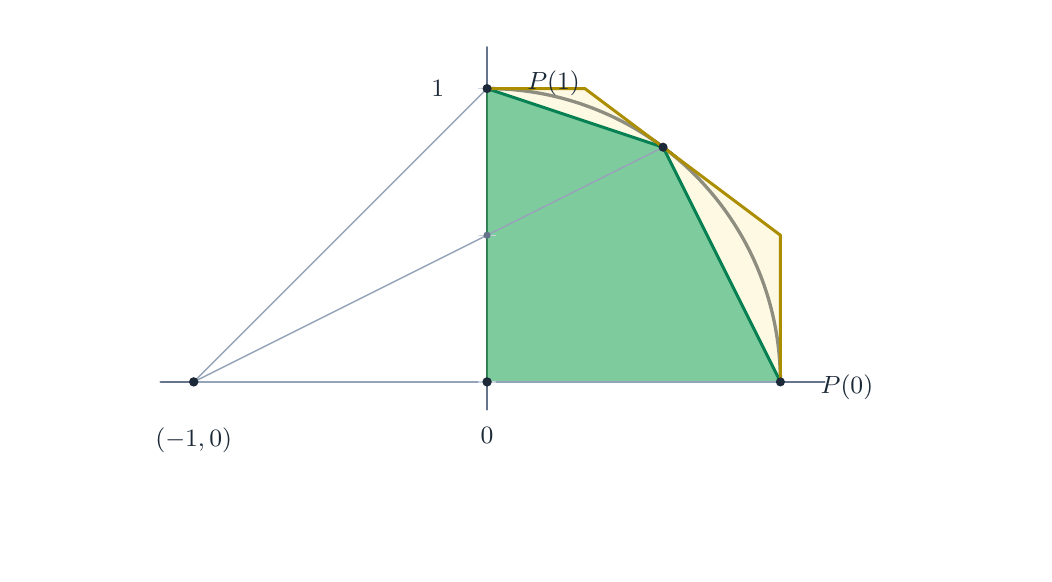
\begin{tikzpicture}[baseline=(current bounding box.north),x=1pt,y=1pt,line cap=round,line join=round]
\useasboundingbox (0,0) rectangle (360,190);
\draw[axis,line width=.75pt] (48,62) -- (288,62);
\draw[axis,line width=.75pt] (166,52) -- (166,183);
\draw[curve,line width=1pt] (166,62) -- (166,168);
\draw[ink,line width=1.2pt] (272,62) arc[start angle=0,end angle=90,radius=106pt];
\path[fill=overfill,fill opacity=.5,draw=over,draw opacity=.8,line width=.45pt] (166,62) -- (272,62) -- (272,115) -- (201.3333,168) -- (166,168) -- cycle;
\path[fill=underfill,fill opacity=.5,draw=under,draw opacity=.8,line width=.45pt] (166,62) -- (272,62) -- (229.6,146.8) -- (166,168) -- cycle;
\draw[projection,line width=.5pt] (60,62) -- (272,62);
\draw[grid,line width=.5pt] (163,62) -- (169,62);
\fill[axis] (166,62) circle[radius=1.3pt];
\draw[projection,line width=.5pt] (60,62) -- (229.6,146.8);
\draw[grid,line width=.5pt] (163,115) -- (169,115);
\fill[axis] (166,115) circle[radius=1.3pt];
\draw[projection,line width=.5pt] (60,62) -- (166,168);
\draw[grid,line width=.5pt] (163,168) -- (169,168);
\fill[axis] (166,168) circle[radius=1.3pt];
\draw[under,line width=1.1pt] plot coordinates {(272,62) (229.6,146.8) (166,168)};
\draw[over,line width=1.1pt] plot coordinates {(272,62) (272,115) (201.3333,168) (166,168)};
\fill[ink] (272,62) circle[radius=1.65pt];
\fill[ink] (229.6,146.8) circle[radius=1.65pt];
\fill[ink] (166,168) circle[radius=1.65pt];
\fill[ink] (166,62) circle[radius=1.7pt];
\fill[ink] (60,62) circle[radius=1.7pt];
\node[font=\small,text=ink,anchor=north] at (60,49) {$(-1,0)$};
\node[font=\small,text=ink,anchor=north] at (166,49) {$0$};
\node[font=\small,text=ink,anchor=east] at (154,168) {$1$};
\node[font=\small,text=ink,anchor=west] at (283,60) {$P(0)$};
\node[font=\small,text=ink,anchor=west] at (177,170) {$P(1)$};
\end{tikzpicture}
\end{document}
